\section{Hardware Implementation}

We have built a 20-node FlashBoost cluster to explore the capabilities of the
architecture. Figure~\ref{fig:bluedbmcluster} shows the photo of our
implementation.

\begin{figure}[ht]
	\begin{center}
	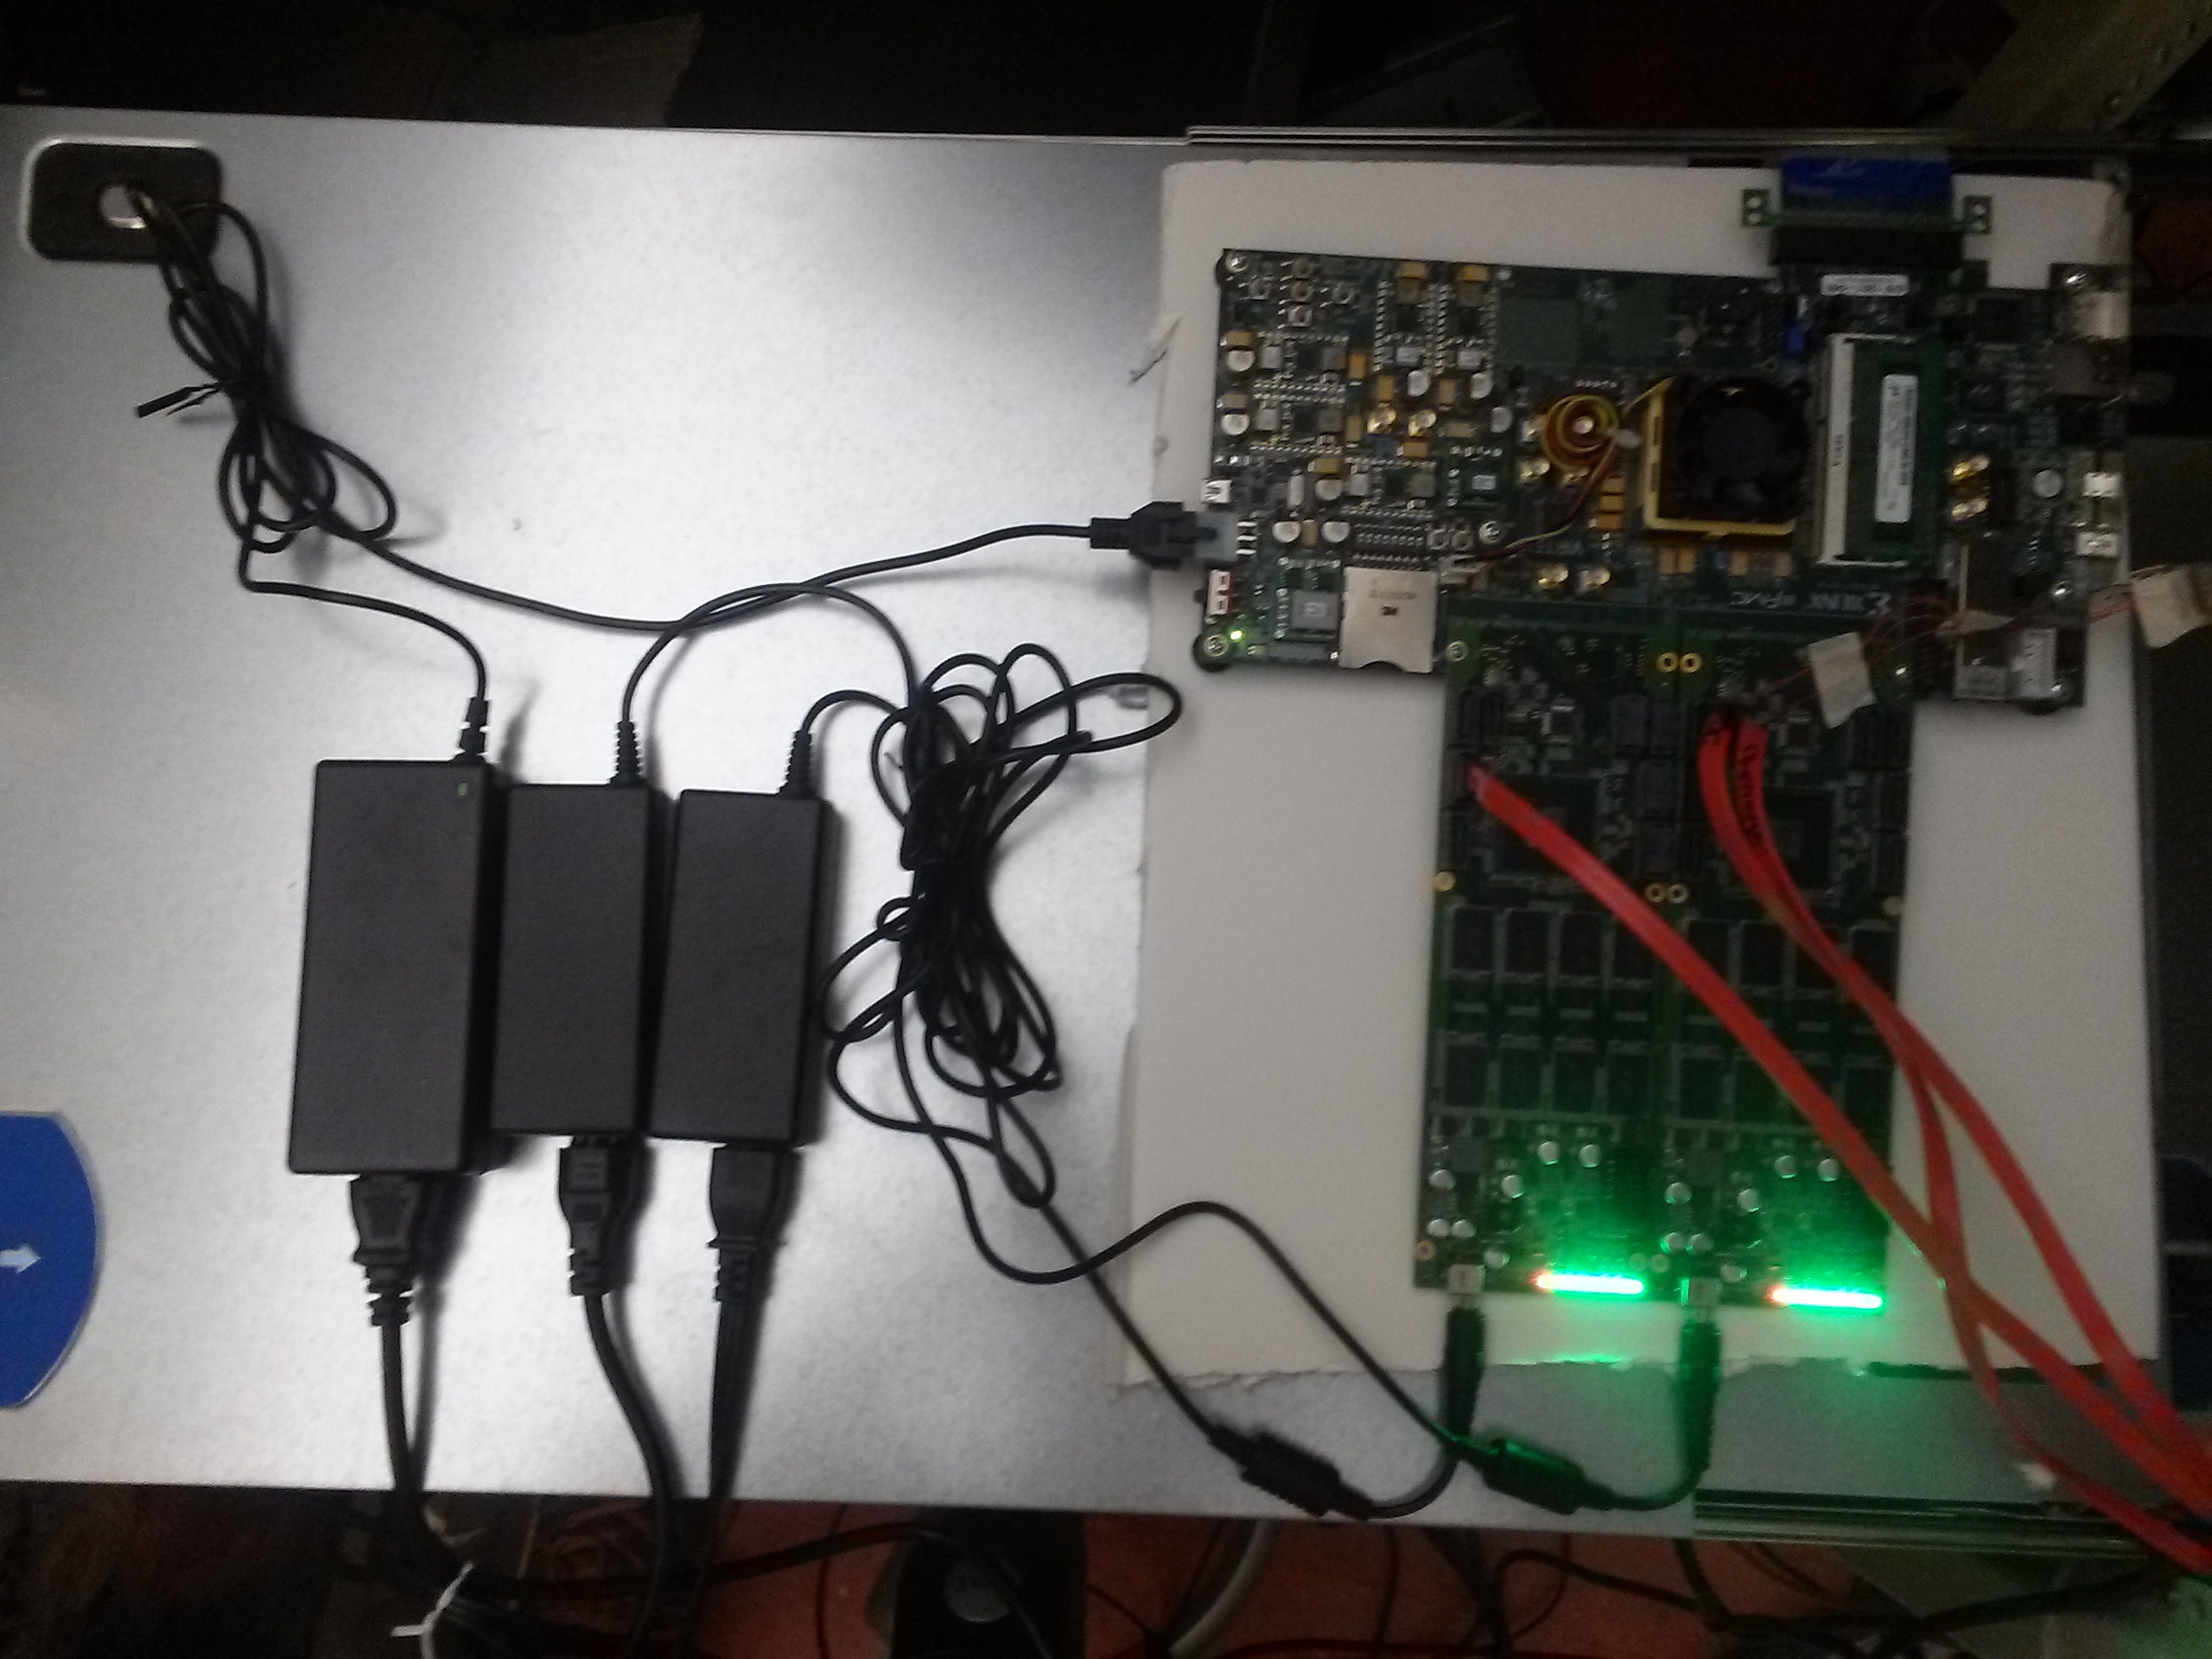
\includegraphics[width=0.3\paperwidth]{figures/rackserver.jpg}
	%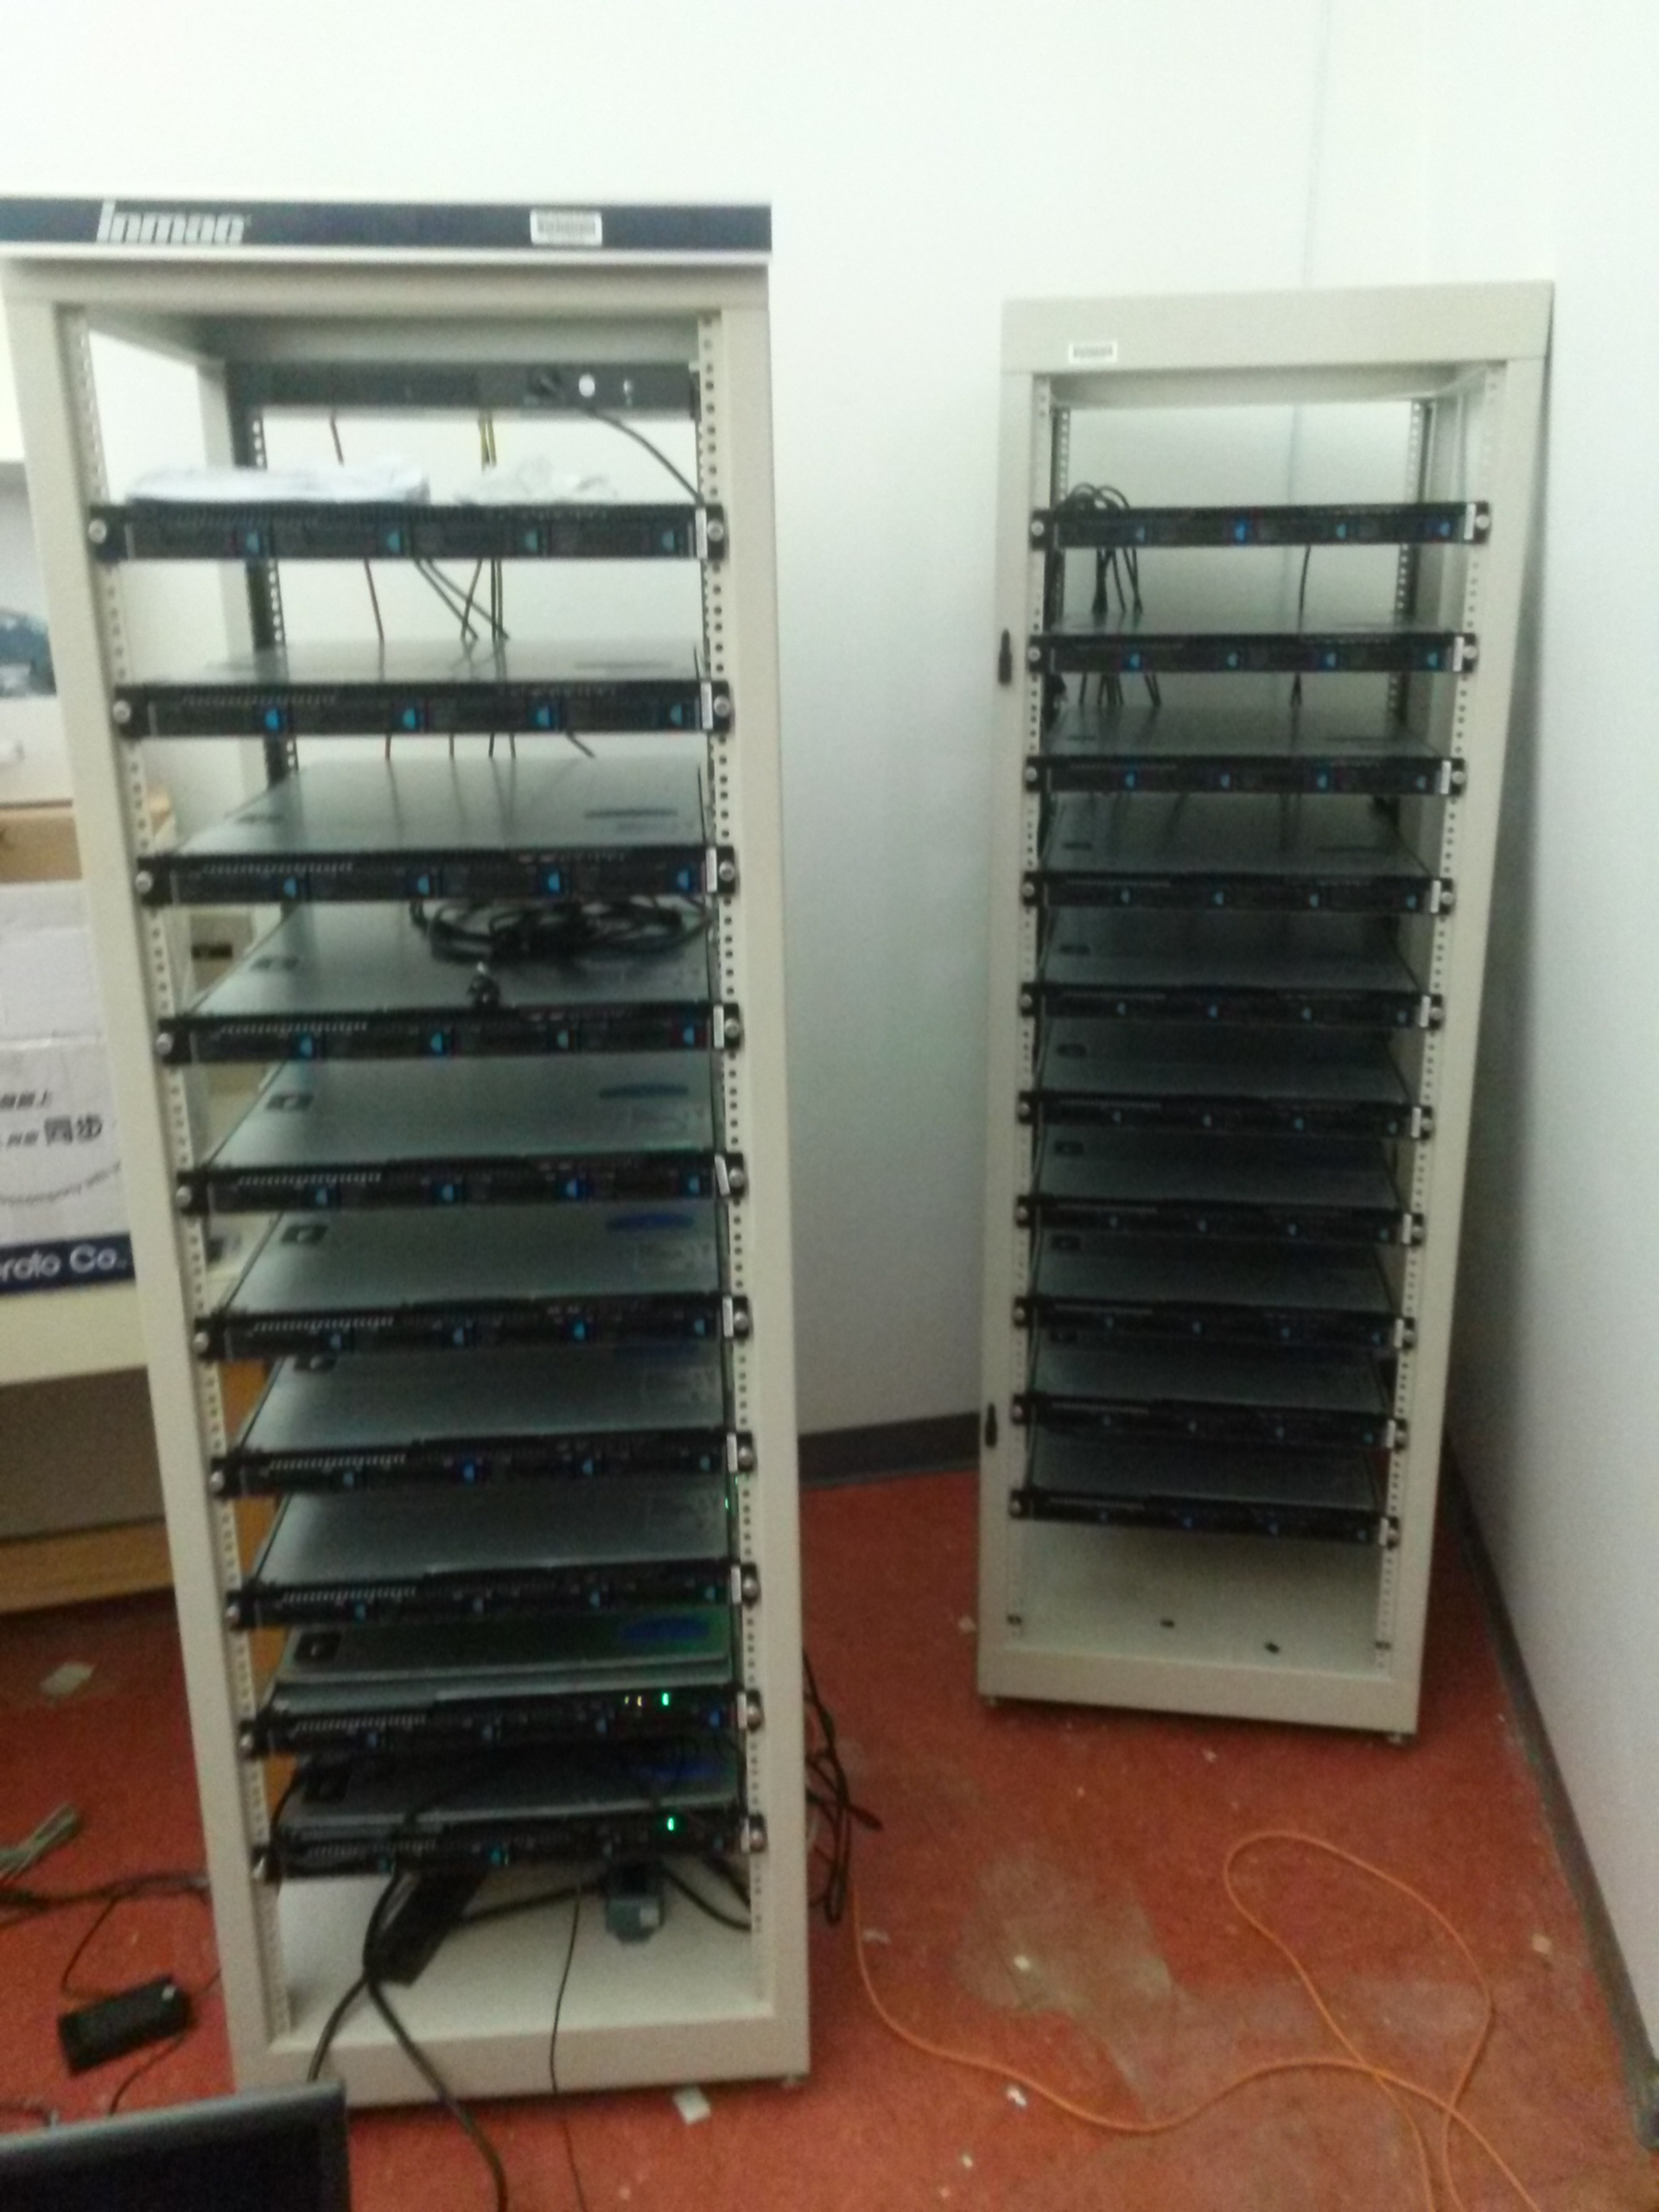
\includegraphics[width=0.3\paperwidth]{figures/rack.jpg}
	\caption{A 20-node FlashBoost Cluster}
	\label{fig:bluedbmcluster}
	\end{center}
\end{figure}

The cluster consists of 20 Xeon servers mounted in two racks, each with a Xilinx
VC707 FPGA development board connected via a PCIe connection. Each VC707 board
hosts two custom-built flash boards with SATA connectors. The VC707 board,
coupled with two custom flash boards is mounted on top of each server.
The host servers run the Ubuntu distribution of Linux.
Figure~\ref{fig:bluedbmnode} shows the components of a single node.

\begin{figure}[ht]
	\begin{center}
	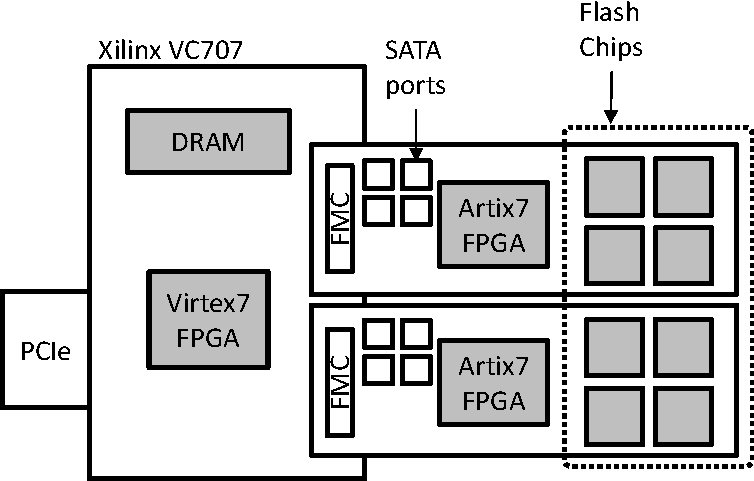
\includegraphics[width=0.4\paperwidth]{figures/storagenode-crop.pdf}
	\caption{A FlashBoost Storage Node}
	\label{fig:bluedbmnode}
	\end{center}
\end{figure}


\subsection{Custom Flash Board}

\begin{figure}[ht]
	\begin{center}
	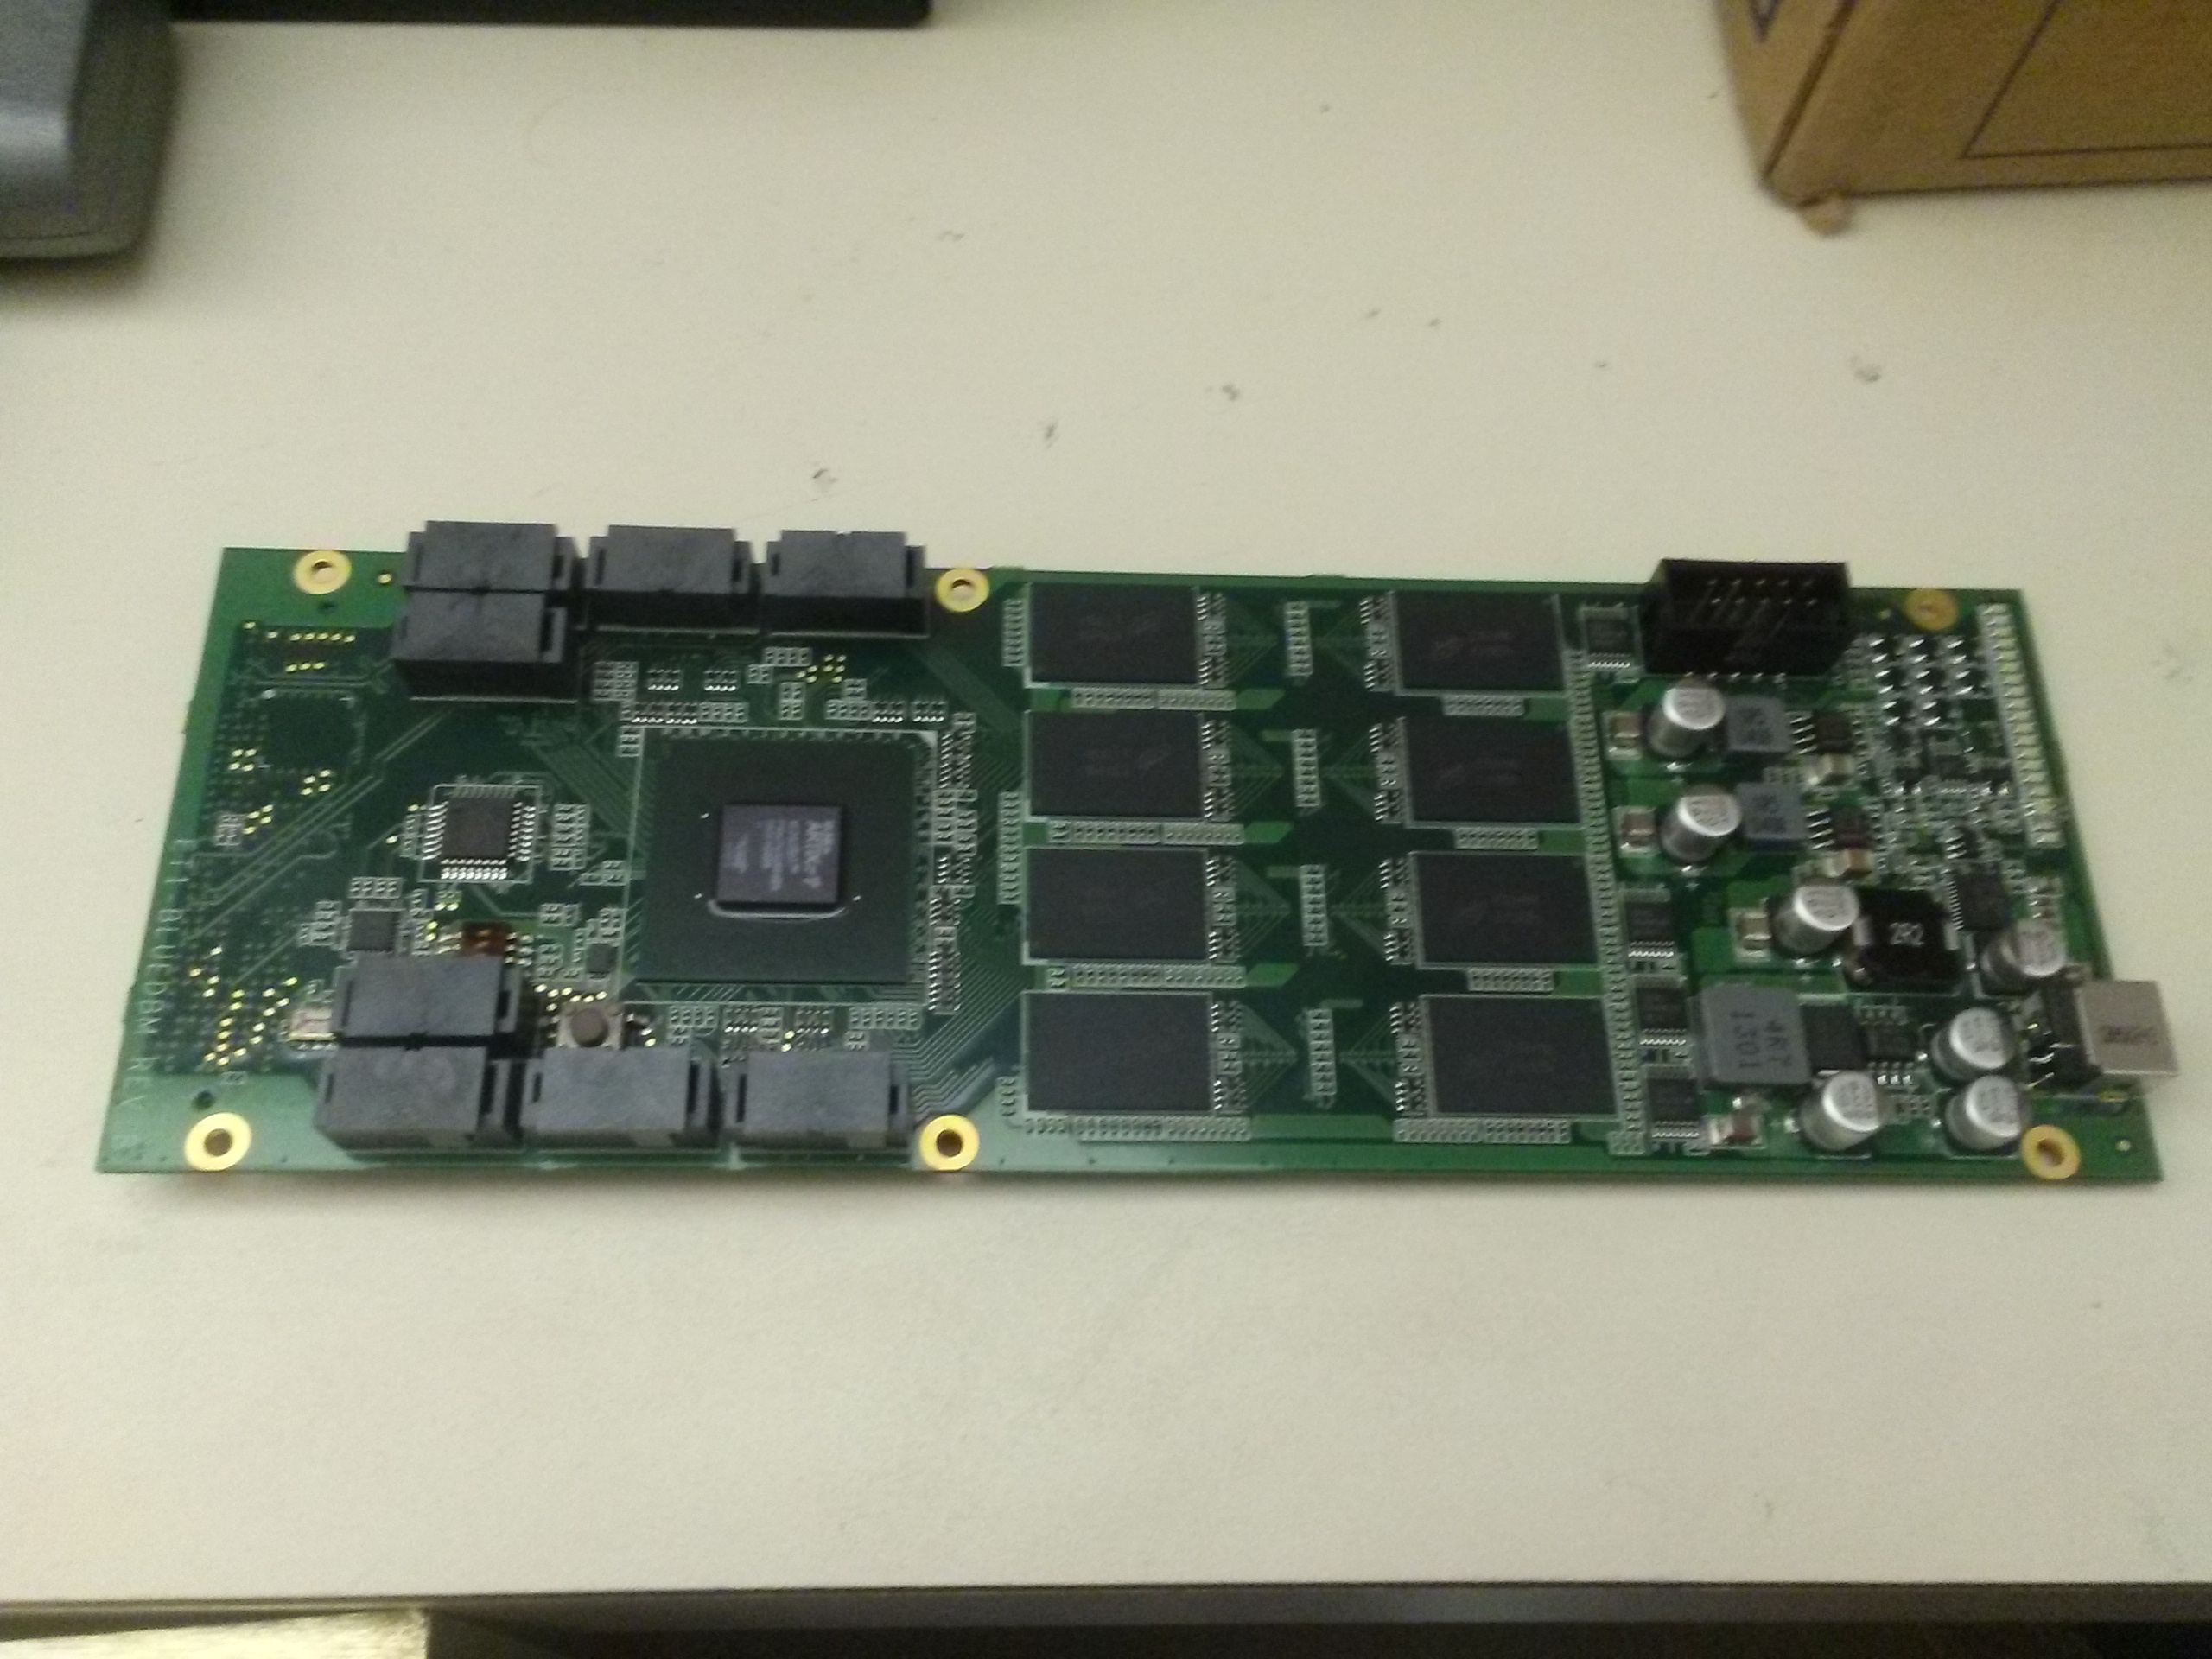
\includegraphics[width=0.4\paperwidth]{figures/flashboard.jpg}
	\caption{A Custom-Built Flash Board with 512GB of NAND Flash}
	\label{fig:flashboard}
	\end{center}
\end{figure}

We have designed and built a high-capacity custom flash board with high-speed
serial connectors, with the help of Quanta Inc., and Xilinx Inc.

Each flash card has 512GBs of NAND flash storage and a Xilinx Artix 7 chip, and
plugs into the host FPGA development board via the FPGA Mezzanine Card (FMC)
connector. The flash controller and Error Correcting Code (ECC) is implemented
on this Artix chip, providing the Virtex 7 FPGA chip on the VC707 a logical
error-free access into flash. The communication between the flash board and the
Virtex 7 FPGA is done by a 4-lane aurora channel, which is implemented on the
GTX/GTP serial transceivers included in each FPGA. This channel can sustain up
to 3.3GB/s of bandwidth at 0.5$\mu s$ latency.
The flash board also hosts 8 SATA connectors, 4 of
which pin out the high-speed serial ports on the host Virtex 7 FPGA,
and 4 of whch pin out the high-speed serial ports on the Artix 7 chip.
The serial ports are capable of 10Gbps and 6.6Gbps of bandwidth, respectively.
